\documentclass{article}
\title{On the length of mature microRNAs}
\author{Dave Tang  \\
	RIKEN Yokohama \\
	\and 
	Derek de Rie \\
	VU University Amsterdam \\
	}

\date{\today}

\usepackage{graphicx}
\graphicspath{ {image/} }
\usepackage{caption}
\usepackage{subcaption}

\usepackage{hyperref}
\hypersetup{
   colorlinks,
   citecolor=black,
   filecolor=black,
   linkcolor=black,
   urlcolor=black
}

\begin{document}

\maketitle

\begin{abstract}
Despite their size, microRNAs (miRNAs) can have dramatic effects on human health due to their direct effect on transcripts. The misregulation of miRNAs can cause a wide spectrum of diseases, such as cancer, and as such they are under heavily investigation.

\end{abstract}

\section{Introduction}

MicroRNAs (miRNAs) were discovered in 1993\cite{pmid8252621} and are the most well known class of non-coding RNAs (ncRNAs).

\section{Methods}\label{method}

All code underlying this work is available at \url{https://github.com/davetang/mirna_length}. Briefly, random sequences were generated using R (version 3.1.0) and the R Bioconductor package Biostrings\cite{biostrings_package}. We generated three sets of one million random sequences that ranged from 15 to 30 base pairs in length, totalling 48 million sequences. The first two sets of sequences were generated based on the multinomial sequence model where each nucleotide in the sequence is independent and identically distributed based on a probability. The first set of randomly generated sequences used an equal probability for each nucleotide ($p_{a} = 0.25$, $p_{c} = 0.25$, $p_{g} = 0.25$, $p_{t} = 0.25$) and the second set used probabilities based on the nucleotide frequency observed in the human genome (hg38): $p_{a} = 0.29$, $p_{c} = 0.20$, $p_{g} = 0.21$, $p_{t} = 0.30$. The third set of randomly generated sequences used a Markov chain model, where the next sequence depends on the previous sequence. Transitions probabilities (Figure ~\ref{fig:transition}) were derived from the dinucleotide frequencies observed from a set of mature human miRNAs downloaded from miRBase\cite{pmid21037258}. The probability of the first base was derived from the frequency of nucleotides at the first base of human mature miRNAs. The alignment of the sequences was performed using BWA\cite{pmid19451168} (version 0.7.9a-r786) using aln/samse and summaries of the mapping were created using Perl scripts. The bar plots were created in R using ggplot2\cite{ggplot2_book} and reshape2\cite{reshape_wickham}.

\begin{figure}[h]
   \centering
   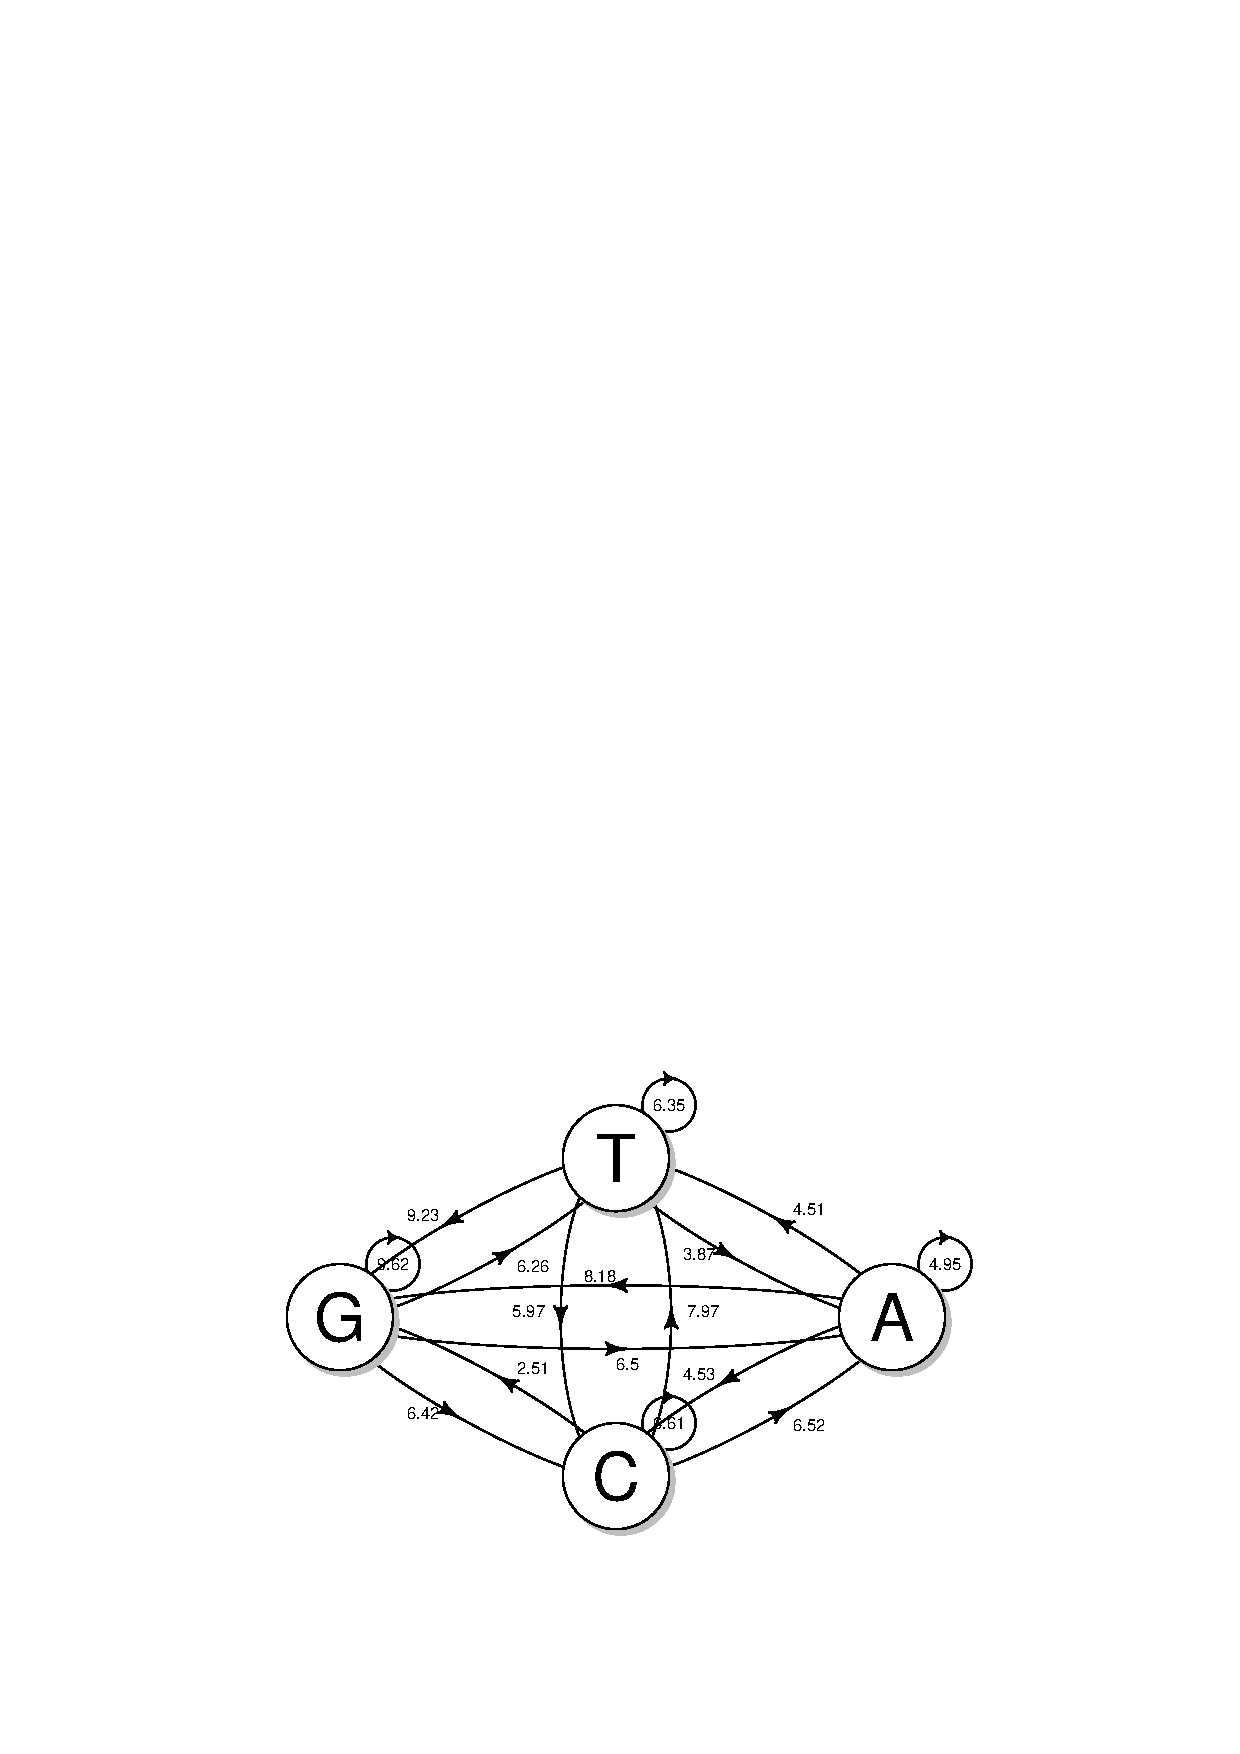
\includegraphics[width=.8\textwidth,natwidth=3297,natheight=2227]{image/transition.png}
   \caption{Transition diagram based on dinucleotide frequencies of miRBase human miRNAs.}
   \label{fig:transition}
\end{figure}

\section{Results}\label{result}

The human genome is mainly composed of repetitive elements, many of which are transposable elements and thus its sequence composition is not a mosaic of random sequences. With this in mind, we would expect that randomly generated sequences would not map back to the human genome. However, it is not known at what length, random sequences will not map back. We investigated this by generating random sequences ranging from 15 base pairs to 30 base pairs under three different models (Section ~\ref{method}) and mapped these sequences to the human genome (Figure ~\ref{fig:mapping}a). At length 18, almost all randomly generated sequences could be mapped to the genome. The number of possible DNA sequences of \textit{n} length is $4^{n}$ and thus a 18 base pair sequence has 68,719,476,736 possible sequences.

\begin{figure}
   \centering
   \begin{subfigure}{.5\textwidth}
      \centering
      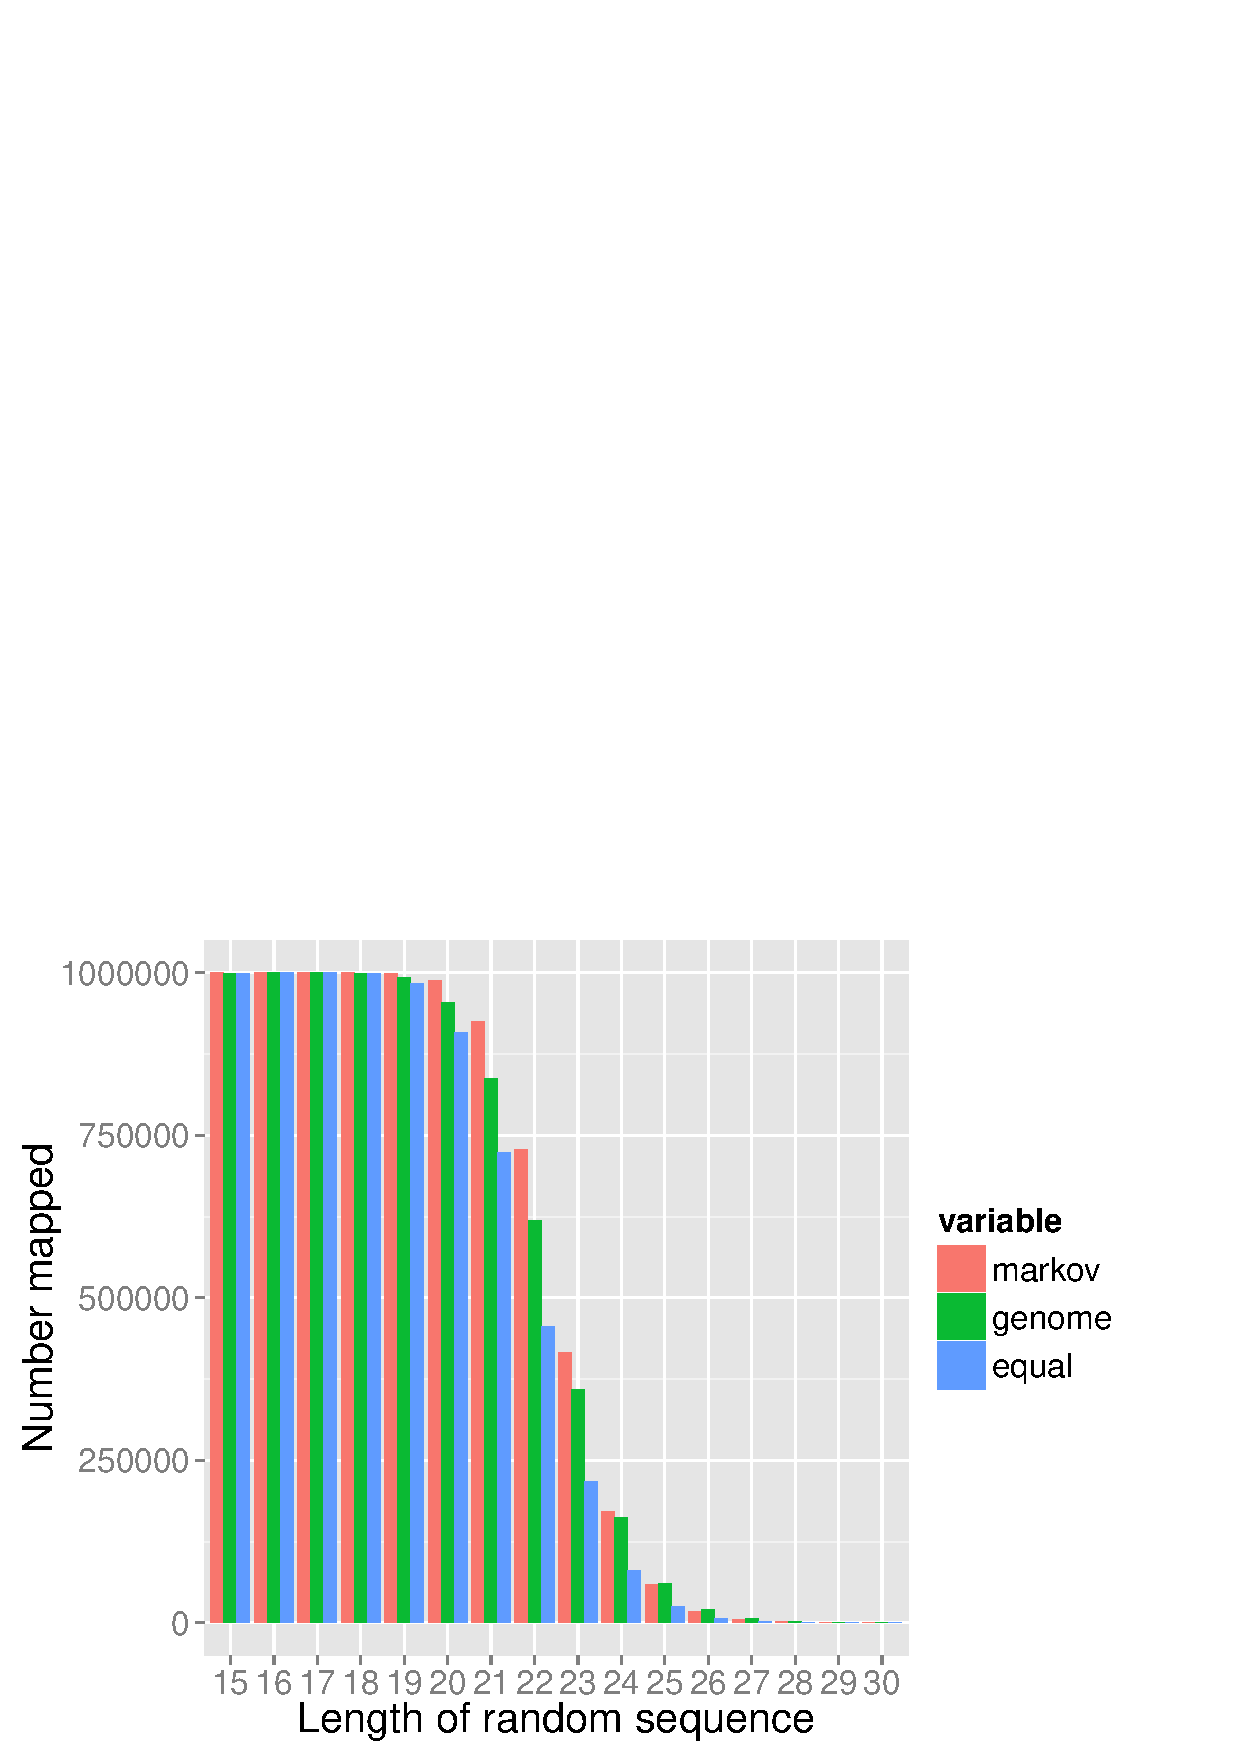
\includegraphics[width=\textwidth,natwidth=2345,natheight=1692]{mapped.png}
      \caption{}
      \label{fig:mapped}
   \end{subfigure}%
      \begin{subfigure}{.5\textwidth}
      \centering
      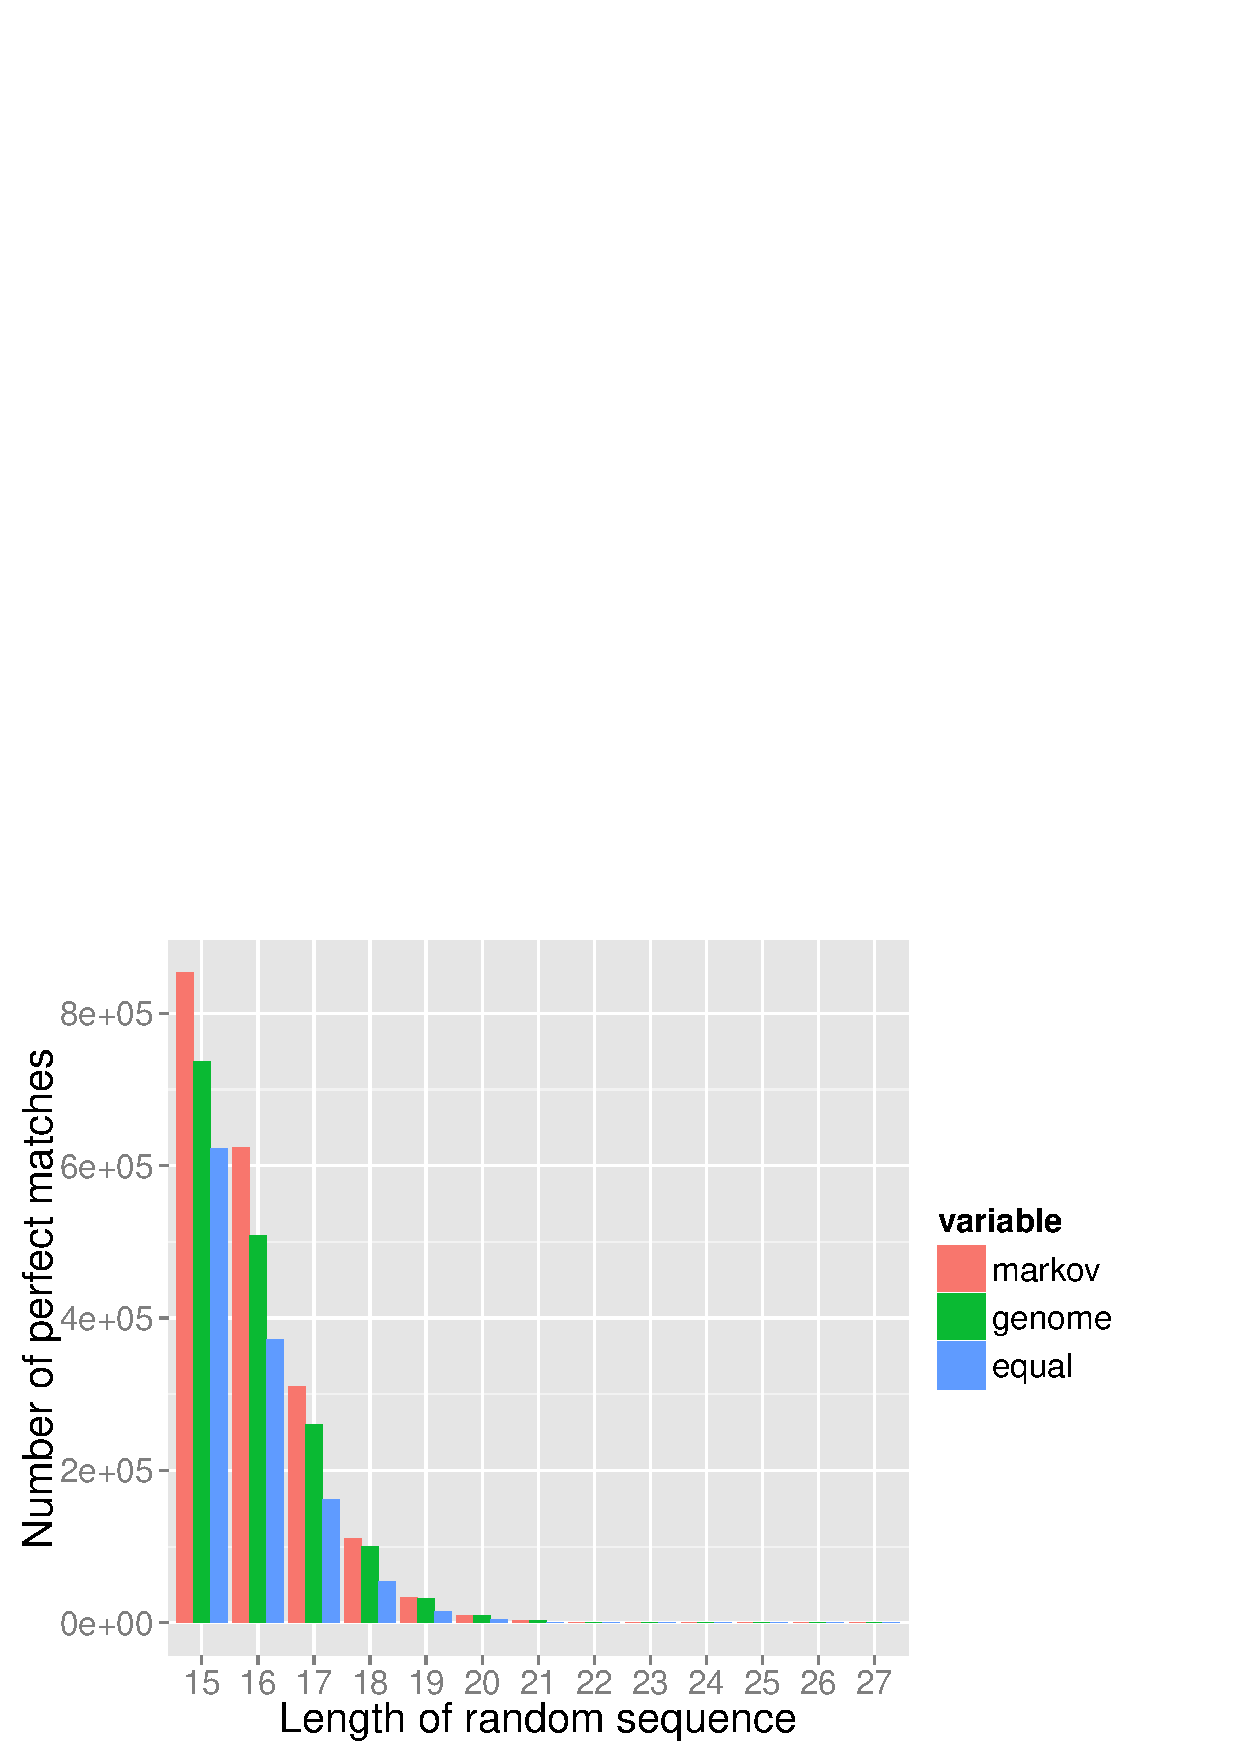
\includegraphics[width=\textwidth,natwidth=2345,natheight=1692]{perfectly_mapped.png}
      \caption{}
      \label{fig:perfect_mapped}
   \end{subfigure}
   \caption{Mapping statistics of three sets of randomly generated sequences. (a) Number of randomly generated sequences mapped back to the human genome. (b) Number of randomly generated sequences perfectly mapped, i.e. mapped without any edits, back to the human genome.}
   \label{fig:mapping}
\end{figure}

\section{Discussion}\label{discussion}

Mammalian miRNAs are able to recognise their target miRNA by as little as 6-8 nucleotides; this region is known as the seed region, which lies at the 5' end of a miRNA. However despite this, most miRNAs are 22-23 base pairs in length.

\bibliographystyle{unsrt}
\bibliography{ref}

\end{document}
